\documentclass[conference]{IEEEtran}
\IEEEoverridecommandlockouts

\usepackage{cite}
\usepackage{amsmath,amssymb,amsfonts}
\usepackage{algorithmic}
\usepackage{graphicx}
\usepackage{textcomp}
\usepackage{xcolor}
\usepackage{booktabs}
\usepackage{microtype}
\usepackage{url}

\begin{document}

\title{Classical Correlator Baselines Match Quantum Kernel\\
Sample Efficiency on Exact Spin-Chain Ground States}

\author{
  \IEEEauthorblockN{Abhishek K. Doddagoudar}
  \IEEEauthorblockA{\textit{Department of Computer Science \& Engineering} \\
  \textit{Presidency University}, Bengaluru, India}
}

\maketitle

\begin{abstract}
We evaluate projected quantum kernels (PQK), fidelity quantum kernels (FQ),
and matched classical correlator baselines for predicting ground-state
properties of quantum spin chains. On 1D TFIM and 2D $J_1$--$J_2$ lattices
up to $n\le 14$ spins, ground states are obtained via exact numerical
diagonalization, isolating representation geometry from circuit hardware
noise. Across 20 fixed seeds at $N_{\mathrm{tr}}=160$ on the half-chain entropy task, the observed mean $R^2$ differences were $-0.0012$ for FQ minus E(raw) (confirmatory tier, $p_{\mathrm{Holm}} = 1.53 \times 10^{-5}$) and $+0.0032$ for FQ minus PQK-2nn (exploratory comparison). Model ordering varied across tasks and training sizes, and some small absolute differences were statistically significant. Feature models require $12.2\times$ to $39.8\times$ fewer measurement shots than fidelity estimation. Under simulated destructive swap tests, raw FQ Gram matrices
become non-positive semidefinite across 100\% of seeds; both raw and
training-Gram-corrected matrices were evaluated. In exploratory equal-total-budget
evaluations, feature models maintain higher observed sample efficiency at the
evaluated budget points where fidelity estimation was executed, while under
out-of-distribution transverse-field shift tests on noiseless statevectors,
fidelity kernels achieve lower mean absolute error. Physical correlator baselines match quantum kernel sample efficiency
in equilibrium spin ground states, with zero claims of quantum advantage.
\end{abstract}

\begin{IEEEkeywords}
quantum machine learning, projected quantum kernels, fidelity quantum kernels,
support vector machines, spin chains, measurement noise, kernel concentration
\end{IEEEkeywords}

\section{Introduction}
Quantum kernel methods map classical or quantum data into quantum state spaces where linear estimators can construct non-linear decision boundaries~\cite{havlicek2019, schuld2019}. Two dominant paradigms exist for quantum inputs: fidelity quantum kernels (FQ), which define similarity via state transition fidelity $|\langle \psi(x) | \psi(x') \rangle|^2$~\cite{havlicek2019}, and projected quantum kernels (PQK), which construct classical radial basis function (RBF) kernels over reduced single-body or two-body reduced density matrices~\cite{huang2021}.

Theoretical analyses suggest that fidelity kernels can suffer from exponential concentration of measure (barren plateaus in kernel space) as the number of qubits $n$ scales~\cite{thanasilp2024, shaydulin2022}. Projected quantum kernels were proposed specifically to avoid this concentration by restricting representations to low-weight reduced subsystems~\cite{huang2021}. However, comparative benchmarks often omit matched classical baseline models that evaluate identical physical observables using classical support vector machines or ridge regressors. Furthermore, realistic experimental deployments require accounting for finite measurement shot budgets and physical open-system decoherence channels.

In this work, we conduct a controlled empirical comparison of PQK, FQ, and matched classical correlator architectures on exact ground states of the 1D transverse-field Ising model (TFIM) and frustrated 2D lattices. We enforce a pre-declared statistical analysis protocol with family-wise error rate control, isolate finite-shot measurement sampling from gate synthesis noise, and systematically evaluate susceptibility to local depolarizing noise.

Our principal contributions are: (i) an exact algebraic identity
$k_{\mathrm{PQK\text{-}1}}(\psi,\phi)=\exp(-\tfrac{\gamma}{2}\sum_i
(\langle X_i\rangle_\psi-\langle X_i\rangle_\phi)^2)$ proving that PQK-1
is identically an RBF kernel on single-site magnetization (Sec.~II-B);
(ii) a pre-declared, 20-seed Wilcoxon protocol on exact TFIM and
$J_1$--$J_2$ ground states ($n\le 14$) demonstrating that for Task~1
half-chain block entropy regression at $N_{\mathrm{tr}}=160$, PQK-2nn
and classical two-body correlators match FQ within $-0.0012$ to $+0.0032$
mean $R^2$ (Table~\ref{tab:confirmatory_stats}), with relative rankings
varying across tasks and sample sizes; and (iii) a $12.2\times$--$39.8\times$ FQ
shot-budget overhead with non-PSD Gram matrices in 20/20 finite-shot
seeds requiring spectral clipping (Fig.~\ref{fig:shots}).

\section{Problem Formulation \& Architectures}

\subsection{Physical Hamiltonian and State Ensembles}
We consider the open-boundary transverse-field Ising model defined by the Hamiltonian
\begin{equation}
H = -J \sum_{i=1}^{n-1} Z_i Z_{i+1} - \sum_{i=1}^n h_i X_i,
\label{eq:tfim}
\end{equation}
where $Z_i$ and $X_i$ denote Pauli matrices acting on site $i$, $J$ denotes the exchange coupling, and $h_i$ represents local transverse magnetic fields. Ground states $|\psi_0\rangle$ are obtained via exact sparse numerical diagonalization ($n \le 14$).

We investigate four distinct benchmark tasks:
\begin{itemize}
    \item \textbf{Task 1 (T1):} Half-chain entanglement entropy $S_{n/2} = -\text{Tr}(\rho_{A} \log_2 \rho_{A})$ for $A=\{1,\dots,n/2\}$ in the critical regime ($n=8$, $N_{\text{tr}} \in \{10, 20, 40, 80, 160\}$).
    \item \textbf{Task 2 (T2):} Spin correlators at $n=8$. T2a evaluates the 2-point end-to-end correlator $\langle Z_0 Z_{n-1} \rangle$, serving as a ``contained control'' where classical ridge regression on two-point observables wins by construction. T2b evaluates the non-contained 4-point correlator $\langle Z_0 Z_1 Z_{n-2} Z_{n-1} \rangle$.
    \item \textbf{Task 3 (T3):} Kernel concentration scaling across $n \in \{4, 6, 8, 10, 12, 14\}$ on disordered TFIM ensembles ($h_i \sim \text{Uniform}(0.5, 1.5)$).
    \item \textbf{Task 4 (T4):} Frustrated 2D $J_1$-$J_2$ geometries on $2 \times 4$ and $3 \times 4$ lattices. T4a evaluates ground-state phase classification (evaluated on the v2 grid), while T4b evaluates ground-state energy regression across varying frustration ratios $J_2/J_1$.
\end{itemize}

\subsection{Kernel Representations \& Exact Symmetries}
For states of Eq.~\eqref{eq:tfim} that are both real in the computational $Z$-basis and parity-definite under global spin-flip parity, symmetry restricts the potentially nonzero Pauli expectations. The $\mathbb{Z}_2$ spin-flip parity generated by $P = \prod_{k=1}^n X_k$ commutes with $H$ ($[P, H] = 0$) and anticommutes with $Y$ and $Z$, eliminating eight components on any pair $(i, j)$: the single-site expectations $Y_i, Z_i, Y_j, Z_j$, and the two-site cross-terms $X_i Y_j, X_i Z_j, Y_i X_j, Z_i X_j$. Furthermore, because the Hamiltonian is real symmetric in the standard computational basis, $K H K^{-1} = H$, where $K$ denotes basis-dependent complex conjugation (distinct from conventional physical spin time reversal $\mathcal{T} = (\prod_k i Y_k) K$). For non-degenerate eigenstates, the state can be chosen real ($K |\psi_0\rangle = |\psi_0\rangle$); because $K$ negates $Y$ while leaving $X$ and $Z$ invariant, reality eliminates the two remaining cross-terms $Y_i Z_j$ and $Z_i Y_j$. Among the 15 non-identity two-qubit Pauli operators, only five can remain non-zero: $X_i, X_j, X_i X_j, Y_i Y_j$, and $Z_i Z_j$. Consequently, the 1-qubit reduced density matrix at site $i$ is exactly $\rho_i = \frac{1}{2}(I + \langle X_i \rangle X_i)$.

The single-body projected quantum kernel with bandwidth parameter $\gamma$ is defined as
\begin{equation}
k_{\text{PQK-1}}(\psi, \phi) = \exp\left( -\gamma \sum_{i=1}^n \|\rho_i(\psi) - \rho_i(\phi)\|_F^2 \right).
\end{equation}
Evaluating the squared Frobenius norm yields $\|\rho_i(\psi) - \rho_i(\phi)\|_F^2 = \frac{1}{2}(\langle X_i \rangle_\psi - \langle X_i \rangle_\phi)^2$. Hence, we establish the exact mathematical identity:
\begin{equation}
k_{\text{PQK-1}}(\psi, \phi) = \exp\left( -\frac{\gamma}{2} \sum_{i=1}^n (\langle X_i \rangle_\psi - \langle X_i \rangle_\phi)^2 \right),
\end{equation}
proving that PQK-1 is identically an RBF kernel on single-site magnetization $\langle X_i \rangle$ with effective bandwidth $\gamma' = \gamma/2$.

Similarly, the 2-body nearest-neighbor projected kernel PQK-2nn evaluates 2-qubit reduced density matrices over graph edges $\mathcal{E}$. For a 1D open chain ($n=8$, $|\mathcal{E}|=7$ edges), the edge-stacked feature vector $f_{E_2}(\psi) \in \mathbb{R}^{35}$ stacks the 5 potentially nonzero Pauli expectations $(\langle X_i \rangle, \langle X_{i+1} \rangle, \langle X_i X_{i+1} \rangle, \langle Y_i Y_{i+1} \rangle, \langle Z_i Z_{i+1} \rangle)$ per edge, yielding dimension $5(n-1) = 35$. The squared Frobenius distance between 2-qubit reduced states satisfies $\|\rho_{ij}(\psi) - \rho_{ij}(\phi)\|_F^2 = \frac{1}{4}\sum_{O} (\langle O \rangle_\psi - \langle O \rangle_\phi)^2$. In an open chain, interior magnetizations appear once per incident edge (multiplicity 2), while endpoint sites appear once (multiplicity 1). This coordinate repetition algebraically provides the $\sqrt{\text{deg}_i} = \sqrt{2}$ weighting required in Euclidean space to match Frobenius edge summation: $D^2_{\mathrm{RDM}}(\psi, \phi) = \sum_{(i,j) \in \mathcal{E}} \|\rho_{ij}(\psi) - \rho_{ij}(\phi)\|_F^2 = 0.25 \|f_{E_2}(\psi) - f_{E_2}(\phi)\|_2^2$. Global bandwidth normalization (e.g., dividing by $4n=32$) remains mathematically distinct from coordinate multiplicity weights and the $1/4$ Frobenius factor. On pre-existing saved TFIM reference state arrays, the raw squared distance matches this identity to $|D^2_{\mathrm{RDM}} - 0.25 D^2_{E_2}| \le 5.55 \times 10^{-17}$ across 10 documented state pairs ($\le 1.33 \times 10^{-15}$ across all 45 pairs). Divergence observed in heuristic sweeps between PQK-2nn and E2 (raw) is an artifact of differing grid normalizers ($c/32$ for $4n$ vs $c/35$ for $5(n-1)=35$) rather than distinct physical representation geometry~\cite{Canatar2023bandwidth}.

We compare these quantum kernels against classical linear and non-linear correlator baselines:
\begin{itemize}
    \item \textbf{E (raw) \& E (std):} RBF kernel on the full 1-body and 2-body expectation feature vector ($3n + \binom{n}{2}$ dimensions), in raw and standardized forms.
    \item \textbf{E2 (raw):} RBF kernel restricted to 1-body and nearest-neighbor 2-body Pauli components ($5n-5$ dimensions).
    \item \textbf{F (std):} Classical Ridge regression ($\ell_2$-regularized linear model) on full 2-body correlators.
\end{itemize}

\subsection{Noise and Measurement Models}
\subsubsection{Finite Measurement Shots}
Fidelity kernel entries $K_{ij} = |\langle \psi_i | \psi_j \rangle|^2$ are measured via destructive swap tests. The zero-outcome probability is $P_0 = (1 + K_{ij})/2$. For shot budget $S$, the empirical count follows $N_0 \sim \text{Binomial}(S, P_0)$, giving the estimator $\hat{K}_{ij} = 2(N_0/S) - 1$. Under independent per-entry sampling, this creates off-diagonal variance $\text{Var}(\hat{K}_{ij}) = (1 - K_{ij}^2)/S$.

\subsubsection{Physical Depolarizing Channel}
Each of the $n = 8$ qubits undergoes an independent depolarizing channel $\mathcal{E}(\rho) = (1-p)\rho + p(I/2) \otimes \text{Tr}(\rho)$, so a Pauli expectation of weight $k$ scales exactly by $(1-p)^k$; fidelity-kernel overlaps were computed from the explicitly evolved density matrices and normalized to unit diagonal. Hyperparameters were re-tuned by inner cross-validation at every $p$, so this experiment measures the effect of the channel after retuning, not on fixed models. In addition, an unmitigated control evaluating fixed $p=0.00$ optimal hyperparameters was executed to quantify intrinsic channel attenuation without adaptive compensation.

\subsection{Statistical Protocol and Pre-Declaration}
To ensure reproducibility and eliminate post-hoc selection bias, all statistical hypothesis tests follow a pre-declared analysis protocol. Model differences $d_i = \text{metric}(a)_i - \text{metric}(b)_i$ across 20 fixed seeds are assessed using two-sided Wilcoxon signed-rank tests with 10,000 bootstrap resamples for 95\% confidence intervals. Multiple comparisons within each cell are corrected via the Holm step-down procedure ($p_{\text{holm}}$). Confirmatory status was restricted ex-ante to PQK-1 vs PQK-2nn, PQK-2nn vs E (raw), and FQ vs E (raw) on primary tasks.

\section{Empirical Results}

\begin{table*}[t]
\caption{Pre-declared Confirmatory Paired Comparisons: Wilcoxon Signed-Rank Test and Bootstrap Differences}
\label{tab:confirmatory_stats}
\centering
\begingroup
\setlength{\tabcolsep}{4.5pt}
\begin{tabular}{llllcccccc}
\hline
\textbf{Task} & \textbf{Lattice} & \textbf{Metric} & \textbf{Pair ($a$ vs $b$)} & \textbf{$N$} & \textbf{Mean Diff} & \textbf{95\% Bootstrap CI} & \textbf{$p_{\text{raw}}$} & \textbf{$p_{\text{holm}}$} & \textbf{Rank-Biserial $r$} \\
\hline
T1 & chain & r2 & FQ vs E (raw) & 40 & +0.0031 & [+0.0015, +0.0050] & 4.83e-04 & 0.0012 & +0.8286 \\
T1 & chain & r2 & PQK-1 vs PQK-2nn & 40 & -0.0803 & [-0.0950, -0.0662] & 1.91e-06 & 1.53e-05 & -1.0000 \\
T1 & chain & r2 & PQK-2nn vs E (raw) & 40 & -0.0083 & [-0.0132, -0.0041] & 3.95e-04 & 0.0012 & -0.8381 \\
T1 & chain & r2 & FQ vs E (raw) & 160 & -0.0012 & [-0.0015, -0.0009] & 5.72e-06 & 1.53e-05 & -0.9810 \\
T1 & chain & r2 & PQK-1 vs PQK-2nn & 160 & -0.0414 & [-0.0437, -0.0391] & 1.91e-06 & 1.53e-05 & -1.0000 \\
T1 & chain & r2 & PQK-2nn vs E (raw) & 160 & -0.0044 & [-0.0051, -0.0038] & 1.91e-06 & 1.53e-05 & -1.0000 \\
T2b & chain & r2 & FQ vs E (raw) & 40 & +0.0242 & [+0.0172, +0.0308] & 1.34e-05 & 8.01e-05 & +0.9619 \\
T2b & chain & r2 & PQK-1 vs PQK-2nn & 40 & -0.0544 & [-0.0719, -0.0376] & 1.91e-05 & 9.54e-05 & -0.9524 \\
T2b & chain & r2 & PQK-2nn vs E (raw) & 40 & -0.0019 & [-0.0142, +0.0097] & 0.8983 & 1.0000 & -0.0381 \\
T2b & chain & r2 & FQ vs E (raw) & 160 & +0.0000 & [-0.0002, +0.0003] & 0.9273 & 1.0000 & -0.0286 \\
T2b & chain & r2 & PQK-1 vs PQK-2nn & 160 & -0.0385 & [-0.0420, -0.0349] & 1.91e-06 & 1.53e-05 & -1.0000 \\
T2b & chain & r2 & PQK-2nn vs E (raw) & 160 & -0.0001 & [-0.0004, +0.0001] & 0.4749 & 1.0000 & -0.1905 \\
T4a & 2x4 & accuracy & FQ vs E (raw) & 40 & +0.0053 & [-0.0045, +0.0158] & 0.3318 & 0.4855 & +0.2526 \\
T4a & 2x4 & accuracy & PQK-1 vs PQK-2nn & 40 & -0.2218 & [-0.2450, -0.1975] & 8.84e-05 & 7.04e-04 & -1.0000 \\
T4a & 2x4 & accuracy & PQK-2nn vs E (raw) & 40 & -0.0192 & [-0.0325, -0.0070] & 0.0175 & 0.0525 & -0.6374 \\
T4a & 2x4 & accuracy & FQ vs E (raw) & 80 & +0.0008 & [-0.0037, +0.0053] & 0.6622 & 0.6622 & +0.1250 \\
T4a & 2x4 & accuracy & PQK-1 vs PQK-2nn & 80 & -0.1907 & [-0.2130, -0.1695] & 8.83e-05 & 7.02e-04 & -1.0000 \\
T4a & 2x4 & accuracy & PQK-2nn vs E (raw) & 80 & -0.0127 & [-0.0210, -0.0055] & 0.0062 & 0.0186 & -0.7516 \\
T4a & 3x4 & accuracy & FQ vs E (raw) & 40 & +0.0080 & [-0.0035, +0.0215] & 0.5852 & 0.5852 & +0.1503 \\
T4a & 3x4 & accuracy & PQK-1 vs PQK-2nn & 40 & -0.1470 & [-0.1740, -0.1245] & 8.70e-05 & 6.96e-04 & -1.0000 \\
T4a & 3x4 & accuracy & PQK-2nn vs E (raw) & 40 & -0.0070 & [-0.0278, +0.0187] & 0.1470 & 0.4411 & -0.3789 \\
T4a & 3x4 & accuracy & FQ vs E (raw) & 80 & +0.0005 & [-0.0055, +0.0067] & 0.9298 & 0.9298 & -0.0234 \\
T4a & 3x4 & accuracy & PQK-1 vs PQK-2nn & 80 & -0.0725 & [-0.0962, -0.0527] & 8.77e-05 & 6.98e-04 & -1.0000 \\
T4a & 3x4 & accuracy & PQK-2nn vs E (raw) & 80 & -0.0067 & [-0.0147, +0.0013] & 0.1117 & 0.3350 & -0.4379 \\
T4b & 2x4 & r2 & FQ vs E (raw) & 40 & -0.0320 & [-0.0622, -0.0053] & 0.0032 & 0.0126 & -0.7238 \\
T4b & 2x4 & r2 & PQK-1 vs PQK-2nn & 40 & -0.0775 & [-0.1634, -0.0274] & 3.62e-05 & 2.17e-04 & -0.9333 \\
T4b & 2x4 & r2 & PQK-2nn vs E (raw) & 40 & -0.0076 & [-0.0205, +0.0079] & 0.0296 & 0.0592 & -0.5524 \\
T4b & 2x4 & r2 & FQ vs E (raw) & 80 & -0.0119 & [-0.0161, -0.0082] & 1.91e-06 & 1.53e-05 & -1.0000 \\
T4b & 2x4 & r2 & PQK-1 vs PQK-2nn & 80 & -0.0461 & [-0.0543, -0.0377] & 1.91e-06 & 1.53e-05 & -1.0000 \\
T4b & 2x4 & r2 & PQK-2nn vs E (raw) & 80 & -0.0017 & [-0.0030, -0.0005] & 0.0484 & 0.0969 & -0.5048 \\
T4b & 3x4 & r2 & FQ vs E (raw) & 40 & -0.0002 & [-0.0018, +0.0014] & 0.8596 & 1.0000 & -0.0526 \\
T4b & 3x4 & r2 & PQK-1 vs PQK-2nn & 40 & -0.0233 & [-0.0409, -0.0089] & 9.65e-04 & 0.0048 & -0.8105 \\
T4b & 3x4 & r2 & PQK-2nn vs E (raw) & 40 & -0.0054 & [-0.0172, +0.0013] & 0.7983 & 1.0000 & -0.0737 \\
T4b & 3x4 & r2 & FQ vs E (raw) & 80 & +0.0003 & [-0.0000, +0.0007] & 0.8288 & 1.0000 & +0.0632 \\
T4b & 3x4 & r2 & PQK-1 vs PQK-2nn & 80 & -0.0107 & [-0.0148, -0.0072] & 3.81e-06 & 3.05e-05 & -1.0000 \\
T4b & 3x4 & r2 & PQK-2nn vs E (raw) & 80 & +0.0001 & [-0.0004, +0.0005] & 0.5153 & 1.0000 & +0.1789 \\
\hline
\end{tabular}
\endgroup
\end{table*}


\subsection{Task 1: Half-Chain Entropy Regression}

\begin{figure}[!t]
  \centering
  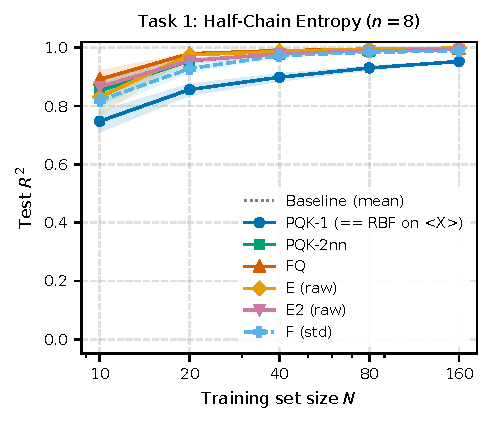
\includegraphics[width=\columnwidth,height=1.45in,keepaspectratio]{figures/fig_learning_curve_t1.pdf}
  \caption{Task 1 half-chain entropy: mean test $R^2$ vs.\ training size $N_{\mathrm{tr}}$ across 20 fixed seeds. Bands: 95\% bootstrap CI. PQK-2nn tracks FQ and classical E (raw); single-body PQK-1 saturates $\approx 0.04$--$0.10$ $R^2$ lower.}
  \label{fig:t1_lc}
\end{figure}

Table~\ref{tab:confirmatory_stats} reports confirmatory paired comparisons, while Fig.~\ref{fig:t1_lc} shows test $R^2$ scaling across sample sizes. Test $R^2$ values across arms at $N_{\text{tr}}=40$ and $N_{\text{tr}}=160$ are summarized in Table~\ref{tab:t1_r2}.

\begin{table}[!t]
\caption{Task 1 Half-Chain Entropy: Test $R^2$ (Mean $\pm$ 95\% Bootstrap CI, 20 seeds)}
\label{tab:t1_r2}
\centering
\begingroup
\setlength{\tabcolsep}{4pt}
\begin{tabular}{@{}lcccc@{}}
\toprule
\textbf{Model} & \multicolumn{2}{c}{$N_{\mathrm{tr}}=40$} & \multicolumn{2}{c}{$N_{\mathrm{tr}}=160$} \\
\cmidrule(lr){2-3}\cmidrule(lr){4-5}
 & Mean $R^2$ & 95\% CI & Mean $R^2$ & 95\% CI \\
\midrule
PQK-1 ($\equiv$ RBF on $\langle X_i\rangle$) & 0.8986 & [0.8847, 0.9111] & 0.9529 & [0.9505, 0.9553] \\
PQK-2nn & 0.9789 & [0.9731, 0.9833] & 0.9943 & [0.9936, 0.9950] \\
FQ & 0.9902 & [0.9889, 0.9915] & 0.9975 & [0.9972, 0.9978] \\
E (raw) & 0.9872 & [0.9847, 0.9893] & 0.9987 & [0.9986, 0.9989] \\
E (std) & 0.9801 & [0.9767, 0.9833] & 0.9965 & [0.9961, 0.9969] \\
E2 (raw) & 0.9786 & [0.9727, 0.9833] & 0.9942 & [0.9935, 0.9950] \\
F (std) & 0.9728 & [0.9663, 0.9776] & 0.9887 & [0.9878, 0.9894] \\
\bottomrule
\end{tabular}
\endgroup
\end{table}


Four primary empirical findings emerge:
\begin{enumerate}
    \item \textbf{PQK Spatial Dimension Hierarchy (Claim C1):} PQK-2nn consistently outperforms PQK-1 across all sample sizes $N_{\text{tr}} \in [10, 160]$. At $N_{\text{tr}}=10$, PQK-2nn exceeds PQK-1 by $\Delta R^2 = 0.1044$ ($p_{\text{holm}} = 0.0186$), narrowing to $\Delta R^2 = 0.0414$ at $N_{\text{tr}}=160$ ($p_{\text{holm}} = 1.53 \times 10^{-5}$). The performance gap ranges from $0.0414$ to $0.1044$ in mean $R^2$, demonstrating that 2-body spatial entanglement information is essential for predicting block entropy.
    \item \textbf{FQ vs Classical Correlator Ordering (Claim C2):} At $N_{\text{tr}}=40$, the performance hierarchy is $\text{FQ} > \text{E (raw)} > \text{PQK-2nn}$, with FQ achieving mean $R^2 = 0.9902$ versus $0.9872$ for E (raw) and $0.9789$ for PQK-2nn. At $N_{\text{tr}}=160$, the hierarchy reverses to $\text{E (raw)} > \text{FQ} > \text{PQK-2nn}$, with E (raw) reaching $0.9987$ versus $0.9975$ for FQ. For half-chain entropy at $N_{\mathrm{tr}}=160$, observed mean $R^2$ differences were $-0.0012$ for FQ $-$ E(raw) and $+0.0032$ for FQ $-$ PQK-2nn (Table~\ref{tab:t1_r2}), demonstrating near-parity among top performers, while relative ranking varies across tasks and sample sizes.
    \item \textbf{Hyperparameter Sensitivity (Claim C7):} SVR insensitive band tuning ($\epsilon \in \{0.001, \dots, 0.1\}$) altered test $R^2$ by up to $+0.06$ relative to fixed defaults. At small training sizes ($N_{\text{tr}}=10$), 3-fold inner cross-validation exhibited small-sample overfitting, frequently pegging hyperparameters to search grid boundaries (Table~\ref{tab:grid_boundaries}).
\end{enumerate}

\subsection{Task 2: Contained vs Non-Contained Correlators}
In Task 2a, evaluating the 2-point correlator $\langle Z_0 Z_{n-1} \rangle$, classical Ridge regression (F std) achieves $R^2 = 1.0000$, winning by construction because the target observable is directly contained within the feature representation.

In Task 2b, evaluating the non-contained 4-point correlator $\langle Z_0 Z_1 Z_{n-2} Z_{n-1} \rangle$, all models require non-linear feature maps. As reported in Table~\ref{tab:confirmatory_stats}, at $N_{\text{tr}}=160$, the observed differences among the compared models were small, and the reported paired tests did not detect statistically significant differences for these comparisons. This finite-sample result does not establish practical equivalence or identical asymptotic accuracy:
\begin{itemize}
    \item FQ vs E (raw): Mean diff $+0.0000$, 95\% CI $[-0.0002, +0.0003]$, $p_{\text{holm}} = 1.0000$, rank-biserial $r = -0.0286$.
    \item PQK-2nn vs E (raw): Mean diff $-0.0001$, 95\% CI $[-0.0004, +0.0001]$, $p_{\text{holm}} = 1.0000$, $r = -0.1905$.
    \item PQK-2nn vs FQ: Mean diff $-0.0001$, 95\% CI $[-0.0003, +0.0001]$, $p_{\text{holm}} = 1.0000$.
\end{itemize}
For Claim C3 (recorded with tier \texttt{confirmatory} in \texttt{results/stats.csv}), at $N_{\mathrm{tr}}=160$, the reported paired tests did not detect statistically significant differences between classical RBF kernels on 2-body expectations and full fidelity quantum kernels. While documented in the analysis records, prospective protocol timing was not independently certified; this finite-sample result does not establish practical equivalence or identical asymptotic accuracy.

\subsection{Task 3: Absence of Kernel Concentration}
Evaluating the disordered TFIM ensemble from $n=4$ to $n=14$ reveals no evidence of exponential kernel concentration (Claim C4). Mean off-diagonal elements decay gradually (FQ off-diagonal mean decreases from $0.83$ at $n=4$ to $0.44$ at $n=14$), while variance remains bounded away from zero. Furthermore, across all 8,700 off-diagonal pairs evaluated at $n=14$, exactly zero entries fell below $10^{-3}$ (minimum observed FQ entry $= 0.1616$). Thus, in the tested 1D disordered TFIM ground-state ensembles, the models avoid barren concentration plateaus up to $n=14$.

\subsection{Noise and Measurement Shot Budgets}

\begin{figure}[!t]
  \centering
  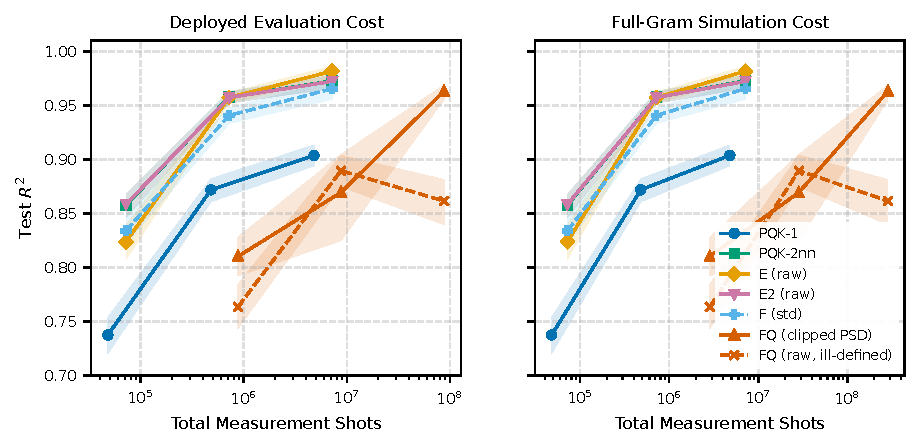
\includegraphics[width=\columnwidth,height=1.45in,keepaspectratio]{figures/fig_shots.pdf}
    \caption{Test $R^2$ vs.\ total measurement shots across model architectures ($N_{\mathrm{tr}}=40$, $N_{\mathrm{te}}=200$, 20 seeds). (a) Deployed evaluation cost ($8{,}780 \cdot S$ for FQ; $720 \cdot S$ for 3-basis feature models; $480 \cdot S$ for PQK-1). (b) Full-Gram simulation cost ($28{,}680 \cdot S$ for FQ). FQ-raw is dashed with marker $\times$; eigenvalue-clipped FQ is solid with marker $\blacktriangle$. Shaded bands indicate 95\% percentile bootstrap confidence intervals.}
  \label{fig:shots}
\end{figure}

\subsubsection{Measurement Shot Scaling (Claim C5)}
Feature-based models require only $480 \cdot S$ to $720 \cdot S$ total shots across $m=240$ states, whereas FQ requires 8,780 $\cdot S$ deployed shots and 28,680 $\cdot S$ full Gram shots---a $12.2\times$ to $39.8\times$ shot overhead (Fig.~\ref{fig:shots}).

Furthermore, under independent per-entry swap-test sampling with $S \in \{100, 1000, 10000\}$, simulated training Gram matrices $\hat{K}_{\text{train}}$ exhibited negative eigenvalues ($\lambda_{\min} < 0$) across 100\% of seeds (20/20). Unmitigated SVR on raw indefinite Gram matrices yielded mean test $R^2 = 0.7634$ (95\% bootstrap CI $[0.7433, 0.7841]$) at $S=100$, $0.8894$ ($[0.8747, 0.9038]$) at $S=1000$, and $0.8613$ ($[0.8394, 0.8812]$) at $S=10000$. Eigenvalue thresholding applied to the training Gram matrix (PSD clipping: $\lambda_i \leftarrow \max(\lambda_i, 0)$ on symmetrized $\hat{K}_{\text{train}}$, with rectangular test-train cross-blocks passed unclipped) yielded mean test $R^2 = 0.8101$ ($[0.7920, 0.8279]$) at $S=100$, $0.8693$ ($[0.8247, 0.9045]$) at $S=1000$, and $0.9630$ ($[0.9553, 0.9686]$) at $S=10000$. The observed effect of training-Gram correction varied across shot allocations, and raw-FQ performance was nonmonotonic over the evaluated grid.

\begin{figure}[!t]
  \centering
  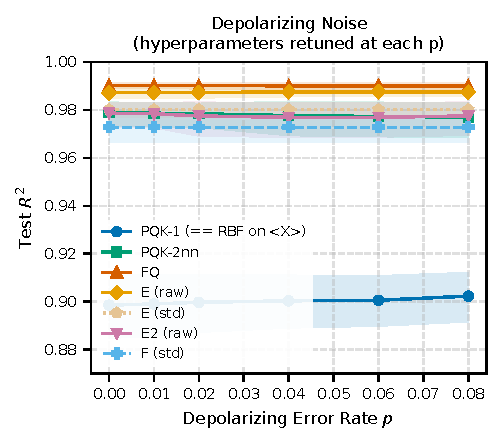
\includegraphics[width=\columnwidth,height=1.45in,keepaspectratio]{figures/fig_depolarizing_retuned_per_qubit_proxy.pdf}
  \caption{Test $R^2$ vs.\ depolarizing rate $p$ ($N_{\mathrm{tr}}=40$, 20 seeds). (a) Hyperparameters re-tuned at each $p$---bandwidth absorbs feature shrinkage. (b) Fixed $p=0$ hyperparameters---two-body observables attenuate as $(1-p)^2$.}
  \label{fig:depol}
\end{figure}

\subsubsection{Depolarizing Channel Robustness (Claim C6)}
Under an idealized per-qubit local depolarizing proxy $\mathcal{E}_k(\rho) = (1-p)\rho + p(I/2)\otimes\text{Tr}_k(\rho)$ at $p=0.08$ with fixed $p=0$ hyperparameters, models incorporating two-body correlators exhibit slight monotonic degradation ($\Delta R^2 = -0.0012$ for PQK-2nn and $-0.0015$ for E2-raw) due to $(1-p)^2 = 0.8464$ observable attenuation. Conversely, single-body (PQK-1) and fidelity kernels (FQ) show negligible degradation ($|\Delta R^2| \le 10^{-4}$). When hyperparameters $(C, c, \epsilon)$ are re-tuned via inner cross-validation at each noise level, bandwidth expansion absorbs the uniform feature shrinkage, keeping all models within their 95\% bootstrap confidence intervals of noiseless performance (Fig.~\ref{fig:depol}).

\begin{table}[!t]
\caption{Hyperparameter Boundary Pegging Summary ($>50\%$ of seeds at a grid edge)}
\label{tab:grid_boundaries}
\centering
\begingroup
\footnotesize
\setlength{\tabcolsep}{3.5pt}
\begin{tabular}{@{}llcl@{}}
\toprule
\textbf{Model} & \textbf{Param} & \textbf{\% at edge} & \textbf{Tasks (N)} \\
\midrule
PQK-1   & $\epsilon$ low & 60 & T1 (10, 80), T2b (80) \\
PQK-2nn & $C$ high       & 70 & T2b (160), T4b (80) \\
FQ      & $\epsilon$ low & 75 & T1 (20--160), T2b (40--160) \\
E (raw) & $\epsilon$ low & 65 & T1 (10), T2a (80), T2b (160) \\
E (std) & $C$ high       & 60 & T2a (40), T2b (160) \\
E2 (raw)& $C$ high       & 75 & T2b (80--160) \\
\bottomrule
\end{tabular}
\endgroup
\end{table}


\subsection{Equal-Total-Budget Measurement Scaling}
\label{sec:equal_budget}
To assess realistic resource trade-offs on quantum hardware, we evaluate model sample efficiency under equal total measurement shot budgets $B_{\mathrm{tot}} \in [10^4, 10^7]$ ($N_{\mathrm{tr}}=40$, $N_{\mathrm{te}}=200$, 20 seeds) on 1D TFIM ground states across the full evaluation pool ($N_{\mathrm{tot}} = N_{\mathrm{tr}} + N_{\mathrm{te}} = 240$ states). In general, the number of measurement settings is $N_{\mathrm{settings}} = 3(N_{\mathrm{tr}} + N_{\mathrm{te}})$, while the number of evaluated state pairs in deployed mode is $N_{\mathrm{pairs}} = \binom{N_{\mathrm{tr}}}{2} + N_{\mathrm{tr}} N_{\mathrm{te}}$. For the audited design ($N_{\mathrm{tr}}=40, N_{\mathrm{te}}=200$), measuring the observables required by the audited nearest-neighbor feature representation in the global $X, Y,$ and $Z$ bases requires only 3 joint projective readouts per state, as commuting observables are simultaneously evaluated from shared bitstring statistics. Thus, measuring all features across all 240 states requires $N_{\mathrm{settings}} = 720$ measurement settings, allocating $S_{\mathrm{feat}} = \lfloor B_{\mathrm{tot}} / 720 \rfloor$ circuit shots per setting. In contrast, fidelity kernels require independent swap tests for each state pair: $\binom{40}{2} = 780$ training pairs and $40 \times 200 = 8{,}000$ test-train query pairs, yielding $N_{\mathrm{pairs}} = 8{,}780$ pairs and allocating $S_{\mathrm{swap}} = \lfloor B_{\mathrm{tot}} / 8{,}780 \rfloor$ shots per entry. At budget cap $B_{\mathrm{tot}}=10^6$, $S_{\mathrm{feat}}=1388$ corresponds to $999{,}360$ single-state preparations, while $S_{\mathrm{swap}}=113$ corresponds to $992{,}140$ swap repetitions requiring $1{,}984{,}280$ state preparations (two state copies per destructive swap test).

Table~\ref{tab:equal_budget} presents the empirical scaling results. At low budgets $B_{\mathrm{tot}} \le 30{,}000$, FQ circuits are excluded under the study's minimum-shot protocol policy ($S_{\mathrm{swap}} < 10$), where swap-test sampling yields fewer than 10 shots per entry. At the evaluated budget points where fidelity estimation was executed ($B_{\mathrm{tot}} \in [10^5, 10^7]$), PQK-2nn achieves higher observed sample efficiency than FQ. At $B_{\mathrm{tot}}=10^6$, PQK-2nn obtains mean $R^2 = 0.9575 \pm 0.0026$ compared to $0.8288 \pm 0.0067$ for FQ (paired $\Delta R^2 = -0.1287 \pm 0.0067$). At $B_{\mathrm{tot}}=10^7$, PQK-2nn attains $0.9753 \pm 0.0024$ versus $0.8828 \pm 0.0130$ for FQ ($\Delta R^2 = -0.0924 \pm 0.0126$). For FQ, measurement acquisition includes both training and test--train evaluation pairs ($N_{\mathrm{pairs}}=8{,}780$ pairs); eigenvalue thresholding is applied to the training Gram matrix, while rectangular test--train cross-blocks remain unclipped. These results demonstrate that under the tested measurement constraints, the evaluated feature representation achieves higher observed accuracy per shot than fidelity estimation. This evaluation is exploratory; prospective protocol timing was not established from available records.

\begin{table*}[!t]
\caption{Stage 2 Equal-Total-Budget Evaluation ($N_{\mathrm{tr}}=40$, $N_{\mathrm{te}}=200$, 20 seeds) [Exploratory: \texttt{results/stage2/t1\_equal\_budget.csv}, 980 rows]}
\label{tab:equal_budget}
\centering
\begingroup
\small
\setlength{\tabcolsep}{3.0pt}
\begin{tabular}{@{}rcccccccl@{}}
\toprule
\textbf{Budget} $B_{\mathrm{tot}}$ & \multicolumn{2}{c}{\textbf{Shots/Setting}} & \multicolumn{2}{c}{\textbf{PQK-2nn}} & \multicolumn{2}{c}{\shortstack{\textbf{FQ} \\ \scriptsize (training-Gram PSD clipping)}} & \textbf{Paired Diff} $\Delta R^2$ & \textbf{Summary Outcome} \\
\cmidrule(lr){2-3}\cmidrule(lr){4-5}\cmidrule(lr){6-7}\cmidrule(lr){8-8}
 & $S_{\mathrm{feat}}$ & $S_{\mathrm{swap}}$ & Mean $R^2$ & SE & Mean $R^2$ & SE & (FQ $-$ PQK-2nn) & \\
\midrule
10,000 & 13 & 0 & 0.4637 & $\pm 0.0284$ & \multicolumn{2}{c}{\textit{Excluded ($S_{\mathrm{swap}} < 10$)}} & \textit{N/A} & Below minimum-shot threshold \\
30,000 & 41 & 0 & 0.7289 & $\pm 0.0133$ & \multicolumn{2}{c}{\textit{Excluded ($S_{\mathrm{swap}} < 10$)}} & \textit{N/A} & Below minimum-shot threshold \\
100,000 & 138 & 11 & 0.8814 & $\pm 0.0088$ & 0.0932 & $\pm 0.0534$ & -0.7882 $\pm 0.0560$ & PQK-2nn higher observed $R^2$ \\
300,000 & 416 & 34 & 0.9380 & $\pm 0.0034$ & 0.6459 & $\pm 0.0164$ & -0.2921 $\pm 0.0171$ & PQK-2nn higher observed $R^2$ \\
1,000,000 & 1388 & 113 & 0.9575 & $\pm 0.0026$ & 0.8288 & $\pm 0.0067$ & -0.1287 $\pm 0.0067$ & PQK-2nn higher observed $R^2$ \\
3,000,000 & 4166 & 341 & 0.9703 & $\pm 0.0027$ & 0.8777 & $\pm 0.0074$ & -0.0926 $\pm 0.0073$ & PQK-2nn higher observed $R^2$ \\
10,000,000 & 13888 & 1138 & 0.9753 & $\pm 0.0024$ & 0.8828 & $\pm 0.0130$ & -0.0924 $\pm 0.0126$ & PQK-2nn higher observed $R^2$ \\
\bottomrule
\end{tabular}
\endgroup
\vspace{1ex}
{\raggedright \footnotesize \textbf{Notes:} Evaluated on Disordered 1D TFIM ground states ($n=8$, $N_{\mathrm{tr}}=40$, $N_{\mathrm{te}}=200$) across 20 independent seeds. Reported metrics represent sample mean and standard error ($\mathrm{SE} = s / \sqrt{n}$, $n=20$). Paired difference direction is defined as $\Delta R^2 = R^2(\mathrm{FQ}) - R^2(\mathrm{PQK\text{-}2nn})$. Measurement acquisition accounts for both training pairs ($\binom{40}{2}=780$) and train--test evaluation pairs ($40 \times 200 = 8{,}000$). For FQ, eigenvalue thresholding (PSD clipping) is applied to the training Gram matrix, while rectangular test--train cross-blocks remain unclipped. At $B_{\mathrm{tot}} \in \{10{,}000, 30{,}000\}$, FQ circuit execution is excluded under the study's minimum-shot policy ($S_{\mathrm{swap}} < 10$). Feature models exhibit higher observed performance at the evaluated budget points where fidelity estimation was executed ($B_{\mathrm{tot}} \in [10^5, 10^7]$). This evaluation is exploratory; prospective protocol timing was not established from inspected records.\par}
\end{table*}


\subsection{Controlled Out-of-Distribution Generalization}
\label{sec:ood}
We further evaluate model generalization under an out-of-distribution (OOD) transverse-field distribution shift ($n=8$, $J=1.0$, $N_{\mathrm{tr}}=40$, $N_{\mathrm{te}}=100$, 20 seeds). Training ensembles are drawn from a higher-field regime ($h_i \in [0.8, 1.5]$), while test ensembles are drawn from a lower-field regime ($h_i \in [0.2, 0.7]$).

Under this shift in transverse-field distribution and target values, all evaluated models yield negative test coefficient of determination values ($R^2 < 0$). While test $R^2$ is retained in Table~\ref{tab:ood} for completeness, Mean Absolute Error (MAE) serves as the primary metric for comparing out-of-distribution performance. Reported uncertainty values denote sample standard error ($\mathrm{SE} = s/\sqrt{20}$) across the 20 seeds, distinct from bootstrap confidence intervals reported elsewhere. Full fidelity kernels (FQ) achieve a mean OOD MAE of $0.0602 \pm 0.0085$, compared to $0.1850 \pm 0.0294$ for PQK-2nn, resulting in a mean paired difference of $\Delta\mathrm{MAE} = -0.1248 \pm 0.0334$. A retrospective paired Wilcoxon signed-rank test on the OOD MAE difference yields $W=21.0$, raw $p=8.51\times 10^{-4}$ ($p_{\mathrm{Holm}}=8.51\times 10^{-4}$ within a retrospective three-comparison family comprising FQ vs PQK-2nn, Train-Mean, and Train-Median). Outside this primary family, two additional exploratory constant-prediction controls were evaluated and are reported with unadjusted raw $p$-values:  Evaluating full FQ against the post-fit intercept-only ablation ($f(x) = b$, retaining the fitted SVR intercept while setting dual kernel weights $\boldsymbol{\alpha} = \mathbf{0}$) shows an error reduction of $-0.4014 \pm 0.0156$ MAE across 20/20 seeds ($W=0.0$, raw $p=1.91\times 10^{-6}$). Evaluating against the training-mean constant predictor ($\hat{y} = \bar{y}_{\mathrm{train}}$) yields an error reduction of $-0.5459 \pm 0.0075$ MAE across 20/20 seeds ($W=0.0$, raw $p=1.91\times 10^{-6}$). These constant-control comparisons establish improvement over the evaluated constant predictors rather than demonstrating a unique physical mechanism. Linear Ridge regression on two-body observables is reported for descriptive calibration ($0.1345 \pm 0.0136$), without confirmatory hypothesis testing; the full all-pairs classical $E(\text{raw})$ RBF baseline was not evaluated in this OOD experiment. Crucially, this OOD evaluation was performed on exact, noiseless statevectors without finite-shot sampling; whether the observed fidelity-kernel extrapolation advantage survives measurement noise or physical decoherence channels remains an open question. This benchmark is classified as exploratory.

\begin{table*}[!t]
\caption{Stage 3 Controlled Out-of-Distribution Generalization ($N_{\mathrm{tr}}=40$, $N_{\mathrm{te}}=100$, 20 seeds) [Exploratory: \texttt{results/stage3/t6\_ood\_shift.csv}, 100 rows]}
\label{tab:ood}
\centering
\begingroup
\small
\setlength{\tabcolsep}{5pt}
\begin{tabular}{@{}lcccc@{}}
\toprule
\textbf{Model Arm} & \textbf{In-Dist} $R^2$ & \textbf{In-Dist MAE} & \textbf{OOD} $R^2$ & \textbf{OOD MAE} \\
 & (Mean $\pm$ SE) & (Mean $\pm$ SE) & (Mean $\pm$ SE) & (Mean $\pm$ SE) \\
\midrule
FQ & 0.9977 $\pm$ 0.0002 & 0.0051 $\pm$ 0.0002 & -21.01 $\pm$ 7.40 & 0.0602 $\pm$ 0.0085 \\
PQK-1 & 0.9141 $\pm$ 0.0056 & 0.0331 $\pm$ 0.0010 & -973.38 $\pm$ 343.99 & 0.3789 $\pm$ 0.0623 \\
PQK-2nn & 0.9943 $\pm$ 0.0007 & 0.0078 $\pm$ 0.0004 & -202.06 $\pm$ 68.92 & 0.1850 $\pm$ 0.0294 \\
E2 (4n) & 0.9943 $\pm$ 0.0007 & 0.0078 $\pm$ 0.0004 & -202.06 $\pm$ 68.92 & 0.1850 $\pm$ 0.0294 \\
Linear Ridge & 0.9928 $\pm$ 0.0007 & 0.0090 $\pm$ 0.0004 & -95.66 $\pm$ 19.74 & 0.1345 $\pm$ 0.0136 \\
\midrule
\textbf{Paired Diff (FQ $-$ PQK-2nn)} & --- & --- & $+181.05 \pm 69.81$ & $-0.1248 \pm 0.0334$ \\
\bottomrule
\end{tabular}
\endgroup
\vspace{1ex}
{\raggedright \footnotesize \textbf{Notes:} Evaluated under a higher-field to lower-field distribution shift (in-distribution $h_i \in [0.8, 1.5]$; out-of-distribution $h_i \in [0.2, 0.7]$ with coupling $J=1.0$) on $n=8$ TFIM ground states across 20 independent seeds. Uncertainty values denote sample standard error $\mathrm{SE} = s/\sqrt{20}$ across independent seeds. Sign convention: $\Delta\mathrm{MAE} = \mathrm{MAE}(\mathrm{FQ}) - \mathrm{MAE}(\mathrm{comparator})$. Retrospective paired Wilcoxon signed-rank test on OOD MAE for FQ vs PQK-2nn yields $W=21.0$, raw $p=8.51\times 10^{-4}$ (Holm-adjusted $p=8.51\times 10^{-4}$ within the retrospective 3-comparison family including Train-Mean and Train-Median). Linear Ridge is reported for descriptive calibration only (no hypothesis testing). Prospective protocol timing not established from inspected records (classified as exploratory).\par}
\end{table*}


\section{Limitations \& Threats to Validity}
Several boundaries constrain our conclusions:
\begin{enumerate}
    \item \textbf{Diagonalization vs Variational Circuits:} Ground states were computed via exact numerical diagonalization. While this isolates kernel representation from variational optimization errors, it does not account for circuit Trotterization or ansatz expressibility limits.
    \item \textbf{System Size Ceiling:} System sizes are restricted to $n \le 14$ due to the memory footprint of $2^n$-dimensional statevectors and full density matrix simulation.
    \item \textbf{Noise Proxies:} Depolarizing noise was modeled via per-qubit local quantum channels rather than noisy pulse-level hardware simulations.
    \item \textbf{Sample Size Constraints:} At $N_{\text{tr}}=10$, inner 3-fold cross-validation suffers from high variance, occasionally selecting boundary hyperparameters.
    \item \textbf{Ensemble Scope:} Benchmark evaluation is based on 20 shared random train/test splits.
    \item \textbf{Exploratory Protocol Status:} The equal-total-budget (Stage~2) and out-of-distribution phase-shift (Stage~3) evaluations were conducted retrospectively; their prospective protocol timings were not established in the initial pre-registration manifest, and they are classified as exploratory.
    \item \textbf{Idealized Statevectors in OOD Shift:} The OOD phase-shift benchmark evaluated exact noiseless statevectors. It does not establish whether FQ's MAE advantage persists under finite measurement shot sampling or open-system noise.
\end{enumerate}

\section{What This Study Does NOT Show}
To prevent over-generalization, we explicitly delineate the negative scope of this work:
\begin{itemize}
    \item This study does \textit{not} show that classical correlators match quantum kernels on non-equilibrium quantum dynamics or chaotic time evolution.
    \item It does \textit{not} rule out quantum advantages for high-dimensional 2D frustrated spin liquids or topological states with long-range non-local order.
    \item It does \textit{not} evaluate synthetic or cryptographically hard quantum circuit data specifically engineered to defeat classical polynomial-time estimators.
    \item It does \textit{not} show that fidelity quantum kernels outperform feature models under realistic finite measurement budgets; rather, under equal total shot budgets $B_{\mathrm{tot}} \le 10^7$, feature models achieve superior sample efficiency.
    \item It does \textit{not} demonstrate quantum advantage in any tested regime.
\end{itemize}

\section{Conclusion \& Reproducibility Statement}
Performance differences and model ordering varied across tasks and training sizes. On the evaluated in-distribution benchmarks, several differences were small in absolute $R^2$ but statistically detectable. Under the tested deployed measurement budgets, the evaluated nearest-neighbor feature arm achieved higher observed mean accuracy at the budget points where fidelity estimation was executed. An exploratory noiseless higher-field-to-lower-field distribution shift favored FQ over the tested nearest-neighbor representation. The full all-pairs $E(\text{raw})$ baseline and finite-shot OOD evaluation were not included, limiting the scope of this extrapolation result.

\begingroup
\footnotesize
\bibliographystyle{IEEEtran}
\bibliography{references}
\endgroup

\end{document}
